%% V1.0
%% by Gabriel Garcia, gabrcg@gmail.com
%% This is a template for Udacity projects using IEEEtran.cls

%% Be Udacious!

\documentclass[10pt,journal,compsoc]{IEEEtran}

\usepackage[pdftex]{graphicx}    
\usepackage{cite}
\hyphenation{op-tical net-works semi-conduc-tor}


\begin{document}

\title{Map My World Robot}

\author{Hsin-Wen Chang}

\markboth{SLAM project, Robotics Nanodegree Program, Udacity}%
{}
\IEEEtitleabstractindextext{%

\begin{abstract}
This project leverage Real time Appearance Based mapping or RTAB-Map for Simultaneous localization and mapping which is the best solution to develop robots that can map environments in 3D. From RTAB-Map's speed and memory management, its custom developed tools for information analysis and, most importantly, the quality of the documentation. Being able to leverage RTAB-Map with our own robots will lead to a solid foundation for mapping and localization well. For this project we will be using the rtabmap ros package, which is a ROS wrapper (API) for interacting with rtabmap. Loop closure is detected using a bag of worlds approach which is commonly used in vision based mapping.
\end{abstract}

% Note that keywords are not normally used for peerreview papers.
\begin{IEEEkeywords}
Robot, IEEEtran, Udacity, \LaTeX, SLAM.
\end{IEEEkeywords}}

\maketitle
\IEEEdisplaynontitleabstractindextext
\IEEEpeerreviewmaketitle
\section{Introduction}
\label{sec:introduction}

\IEEEPARstart{S}{im}ultaneous localization and mapping (SLAM) is used for constructing and updating a map from unknown environment while keep tracking agent's location. In this project, SLAM was perform on two simulate 3D world where robot can mapping and localize them self by interface the robot with RTAB-Map addition of an RGB-D camera which allows robot estimate their trajectory and map feature pose through explore its environment and create high accuracy map of it's surround environment. The two environment should be mapped in 2D and 3D by using Gazebo and RViz.

\section{Background}
 When a mobile robot is mapping a large environment while traveling in cycles and correlating between different objects will face challenges and difficulties such as Unknown map, huge hypothesis space, size, noise, cycles and perceptual ambiguity. Mapping with know pose. The technologies combine localization and mapping process called Simultaneous localization and mapping (SLAM)\cite{lamport1994latex}

\subsection{Occupancy Grid Mapping}
While listing the different challenges and difficulties in mapping, The words discrete and continuous:

Discrete Data: You obtain this data by counting it. This data has finite values. Example: Number of robots in a room.

Continuous Data: You obtain this data by measuring it. This data has an infinite number of steps, which form a continuum. Occupancy Grid Mapping applied Posterior Probability implement a mapping algorithm and estimate the map given noisy measurements and assuming known poses.

\subsection{Grid-based FastSLAM}
The FastSLAM algorithm solves the Full SLAM problem by following:
%example for Bullet point list
\begin{itemize}
\item Estimating the Trajectory: FastSLAM estimates a posterior over the trajectory by applying particle filter approach which is an advantage to SLAM to solve the problem of mapping with known poses.
\item Estimating the Map: FastSLAM uses a low dimensional Extended Kalman Filter to solve independent features of the map which are modeled with local Gaussian.

The custom approach of representing the posterior with particle filter and Gaussian is known by the Rao-Blackwellized particle filter approach.
\end {itemize}
\begin{figure}[thpb]
      \centering
      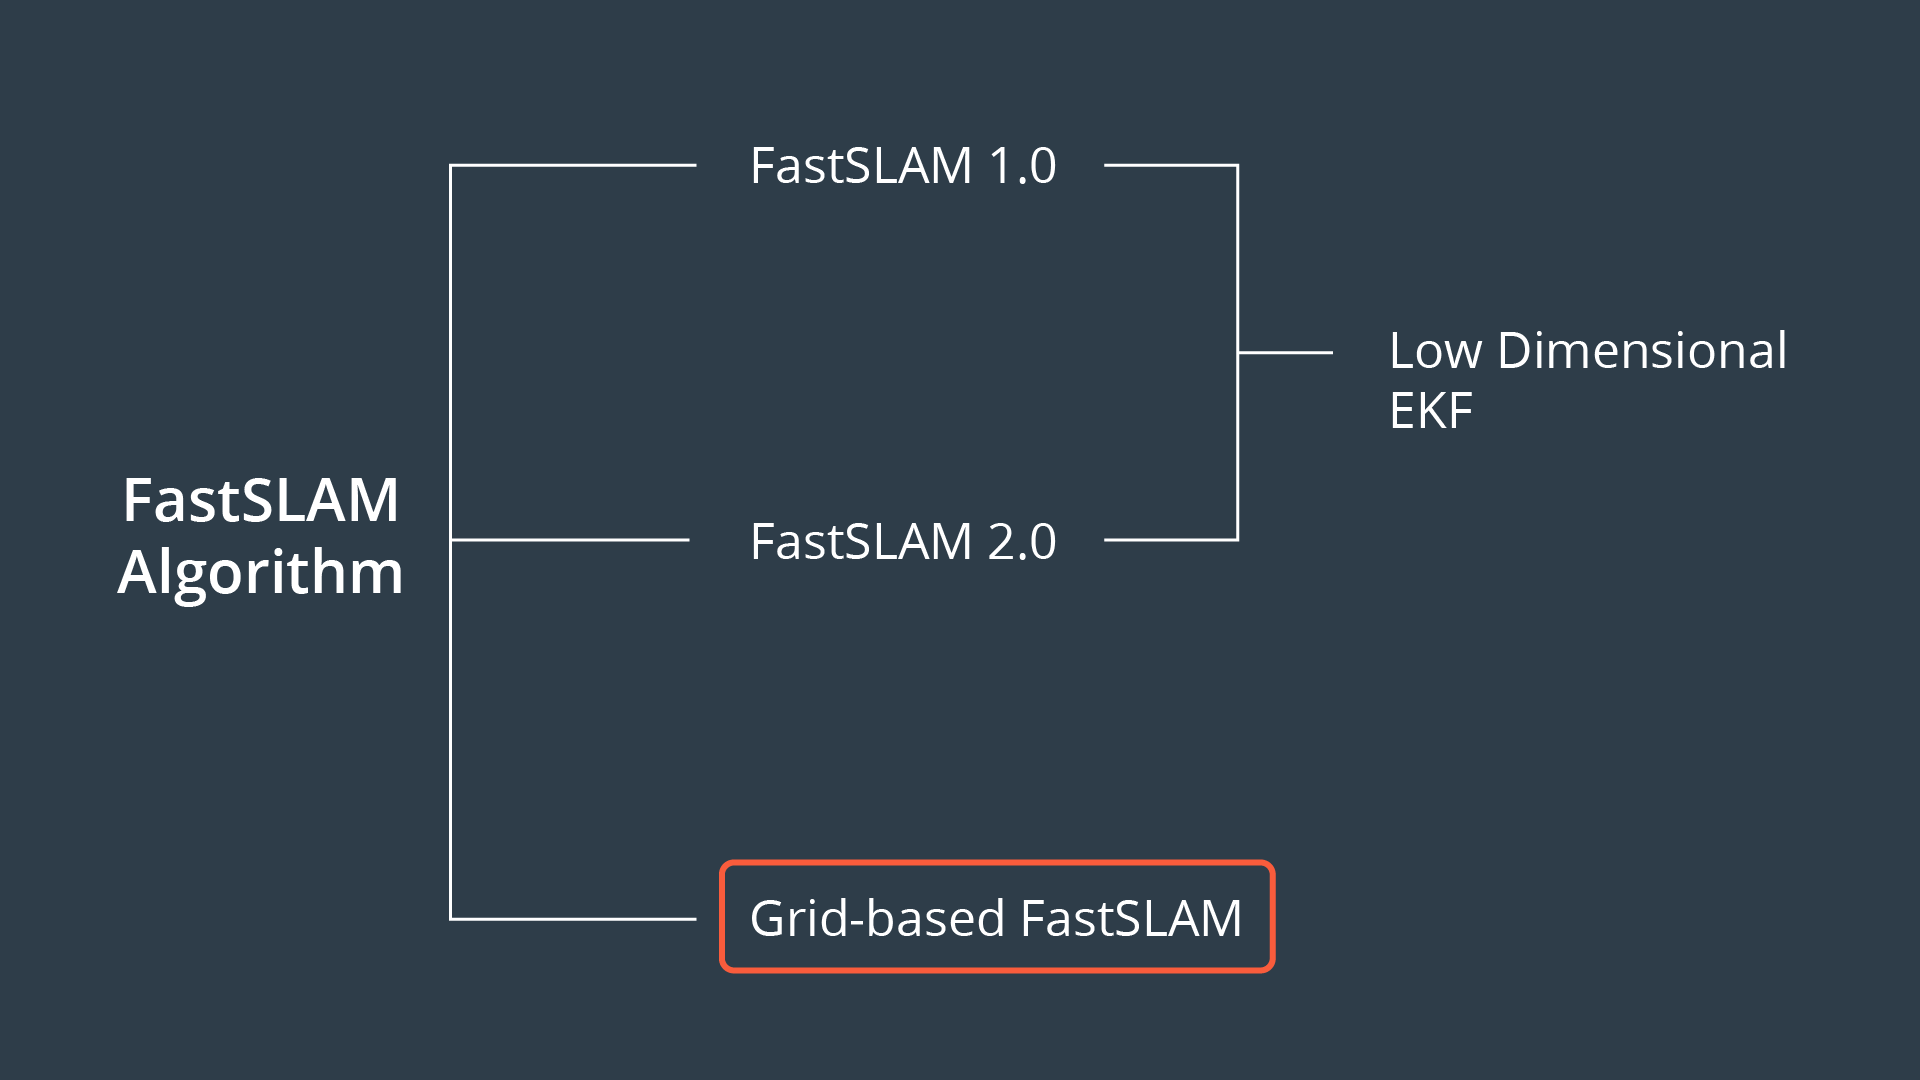
\includegraphics[width=\linewidth]{FastSLAM.png}
      \caption{FastSLAM.}
      \label{fig:robot1}
\end{figure}
\subsection{GraphSLAM}
GraphSLAM is a SLAM algorithm which solve the full SLAM problem and recovers the entire path and map instead of just recent pose and map.At the core of GraphSLAM is graph optimization - the process of minimizing the error present in all of the constraints in the graph by applying maximum likelihood estimation (MLE) to structure and solve the optimization problem for the graph.
In RTAB-Map, loop closure is detected using a bag of worlds approach which is commonly used in vision based mapping.
\begin{figure}[thpb]
      \centering
      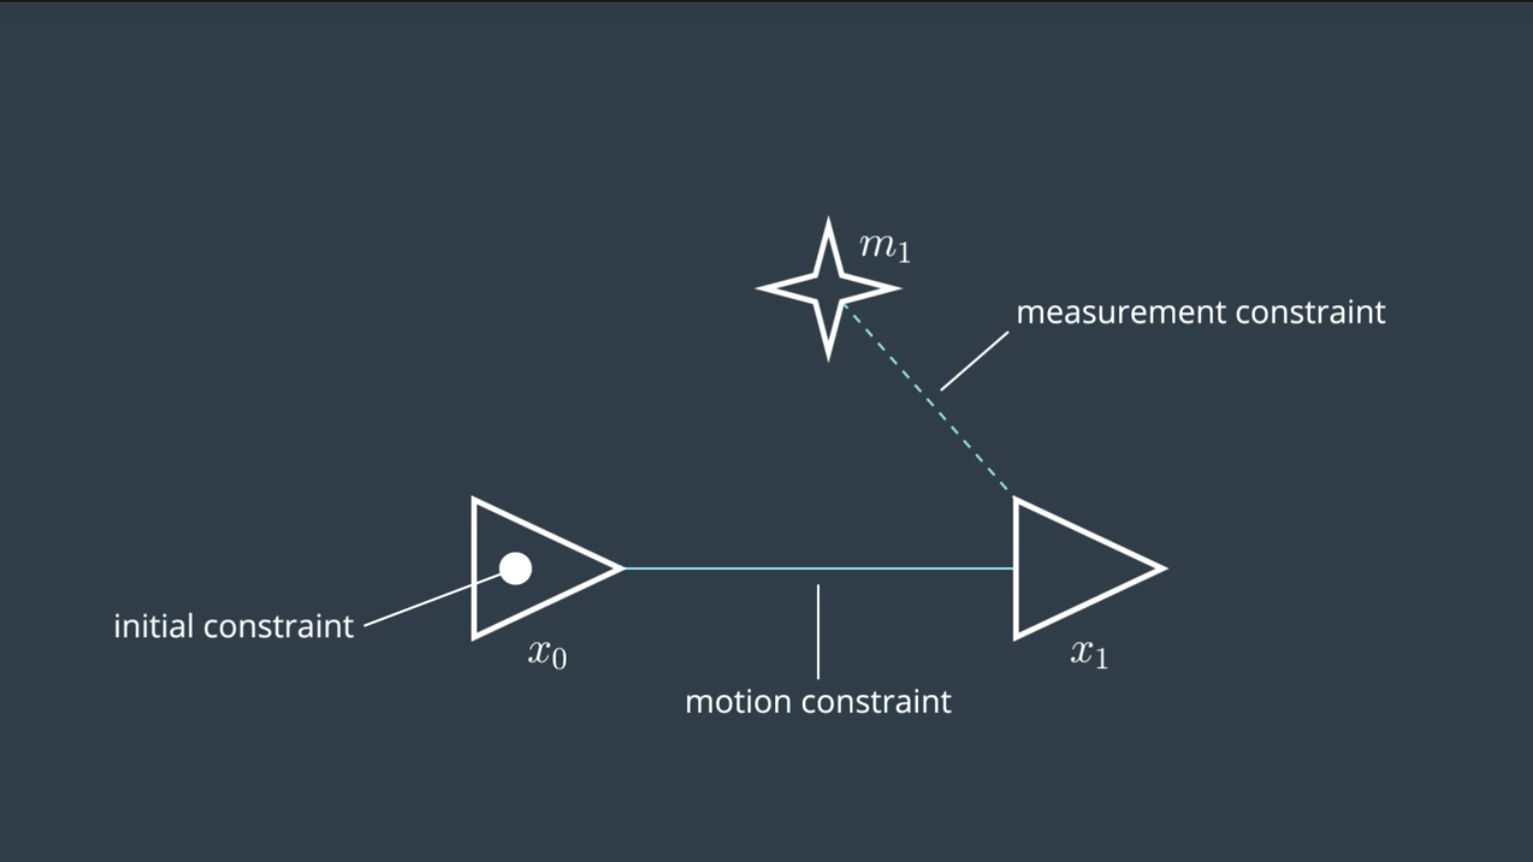
\includegraphics[width=\linewidth]{GraphSLAM.png}
      \caption{GraphSLAM.}
      \label{fig:robot1}
\end{figure}

\section{Scene and robot configuration}

\subsection{Kitchen and dining scene}
The Kitchen and dining scene was provided by Udacity as benchmark scene.
\subsection{My World scene}
You should describe what you achieved for localization in the project with the benchmark model and your own model. Includes charts and graphs show how parameters affect your performance. 
\subsection{Robot configuration: tf tree}
\begin{figure}[thpb]
      \centering
      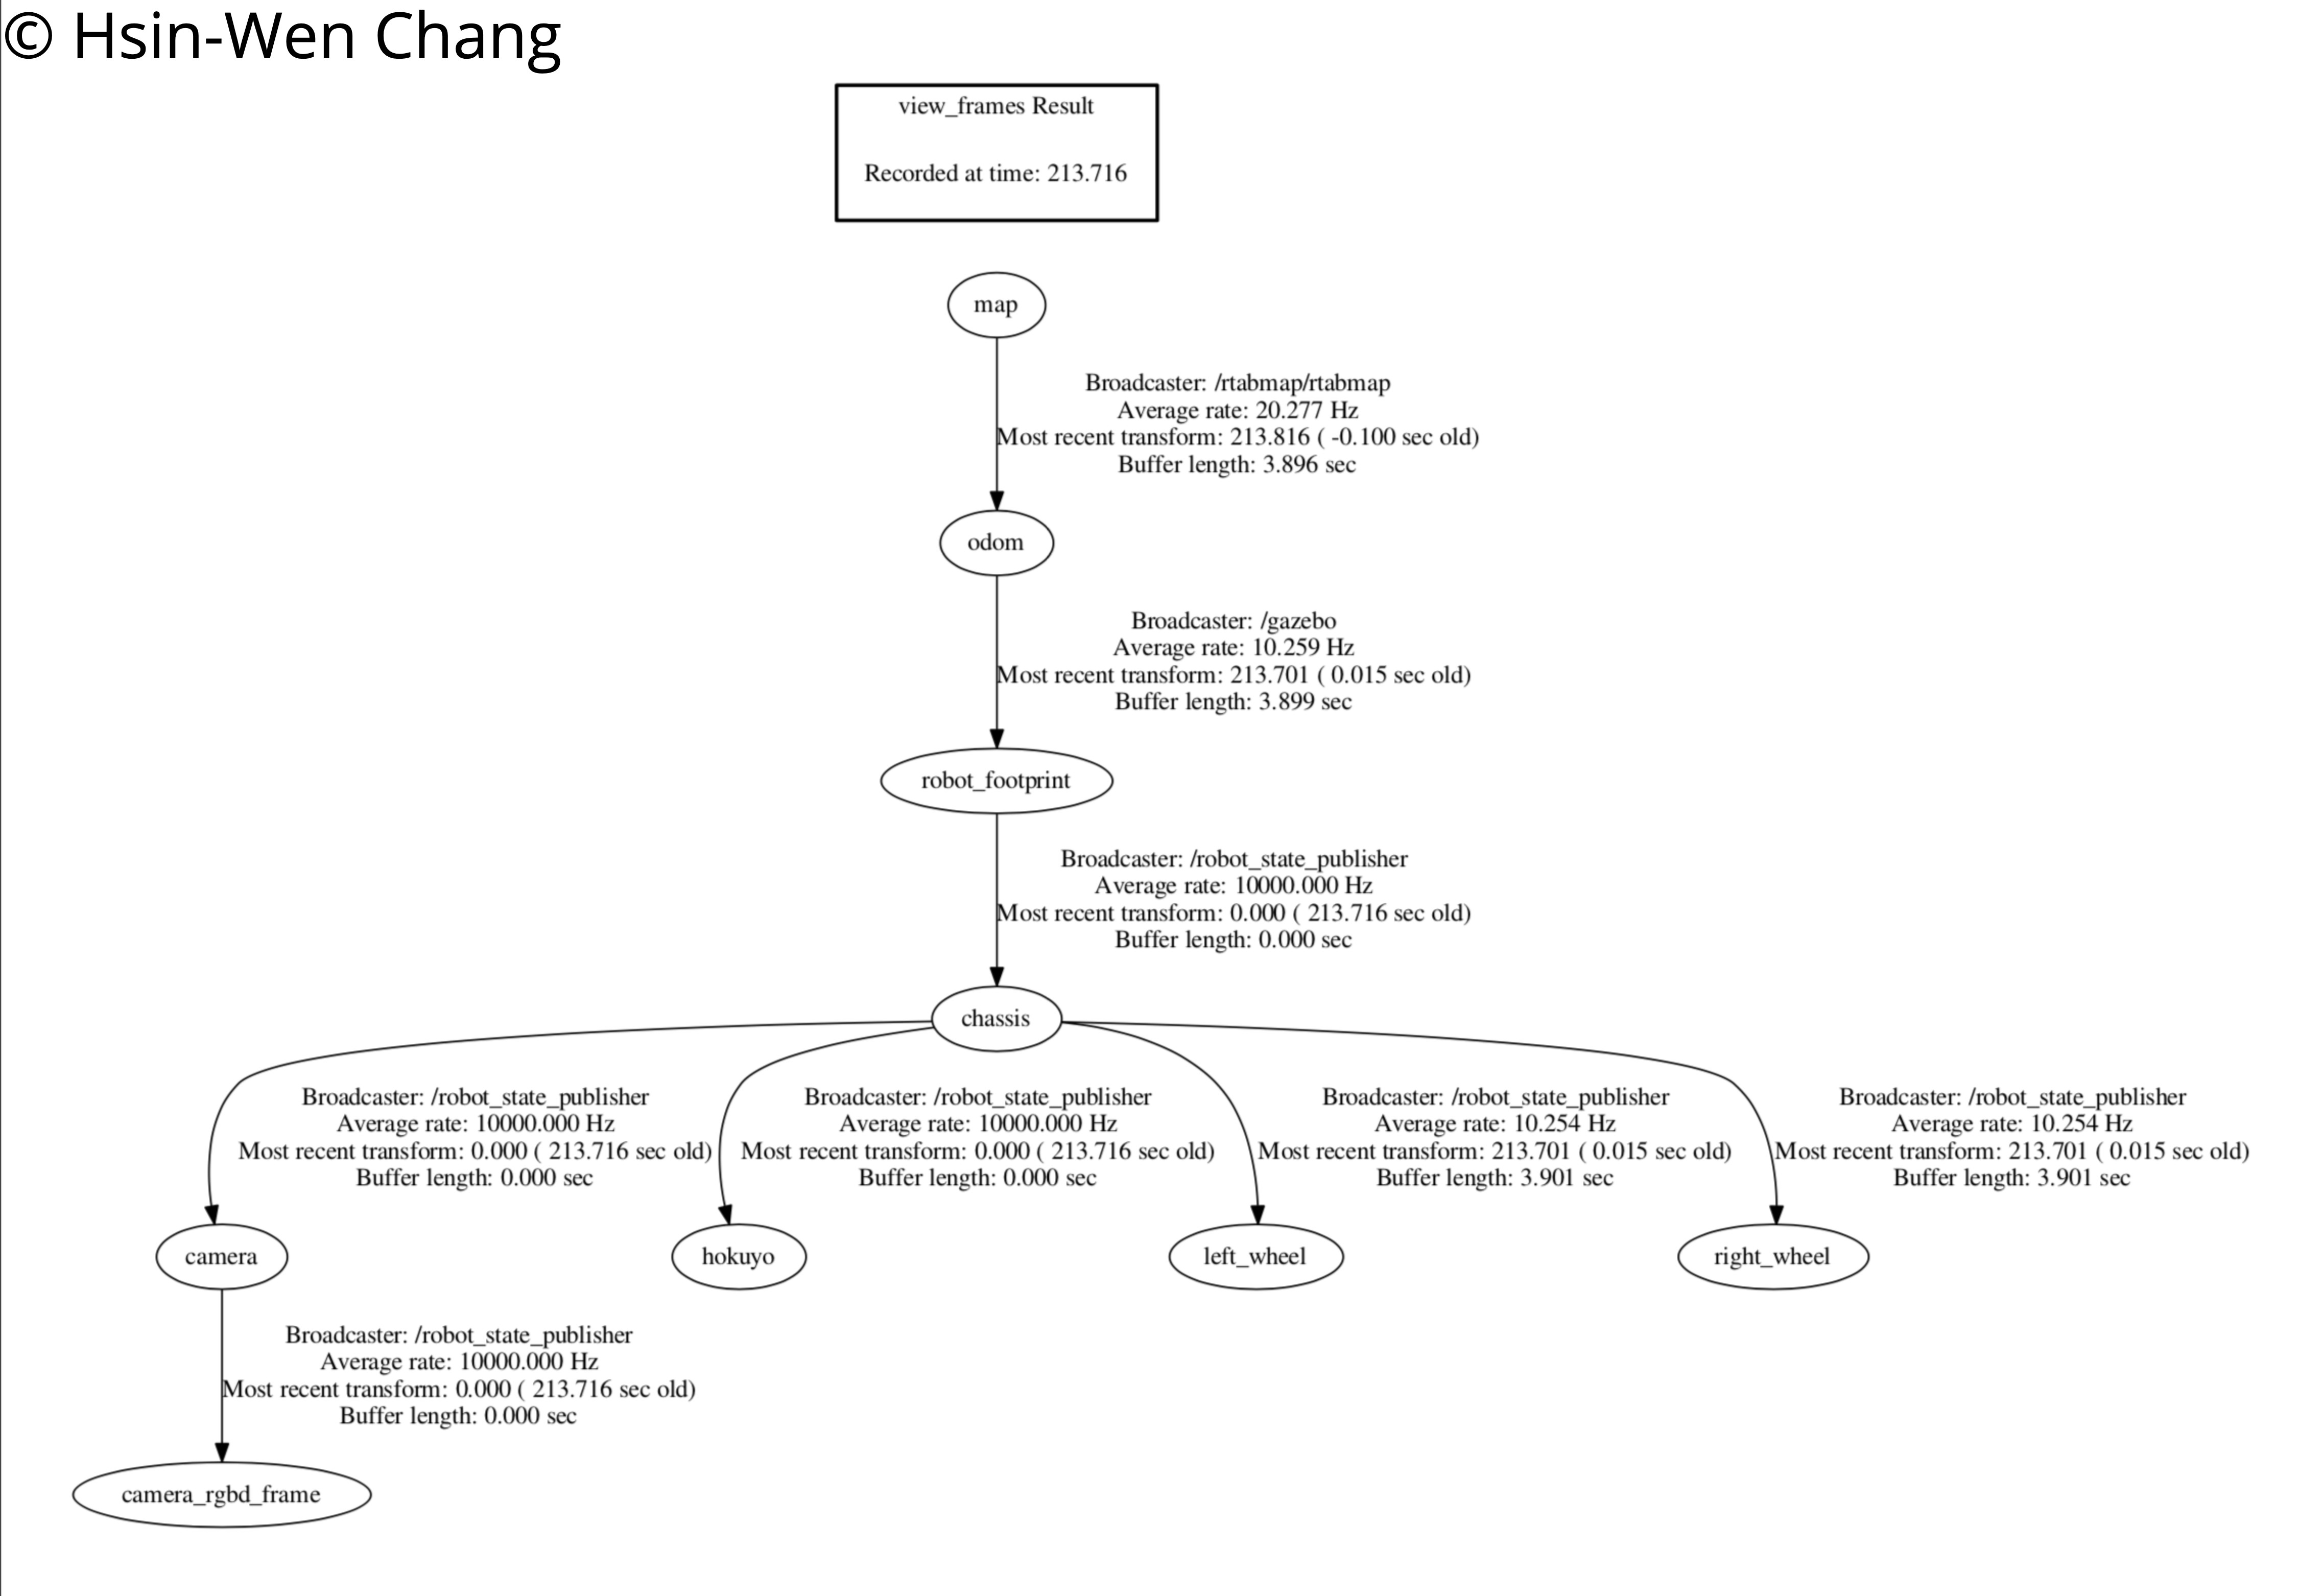
\includegraphics[width=\linewidth]{TransformFrames.png}
      \caption{Robot transformation tree.}
      \label{fig:robot1}
\end{figure}
\section{Results}

\subsection{SLAM Results}
\subsubsection{Kitchen and dining scene}

\subsubsection{My World scene}

\section{Discussion}


\section{Conclusion / Future work}

\begin{figure}[thpb]
      \centering
      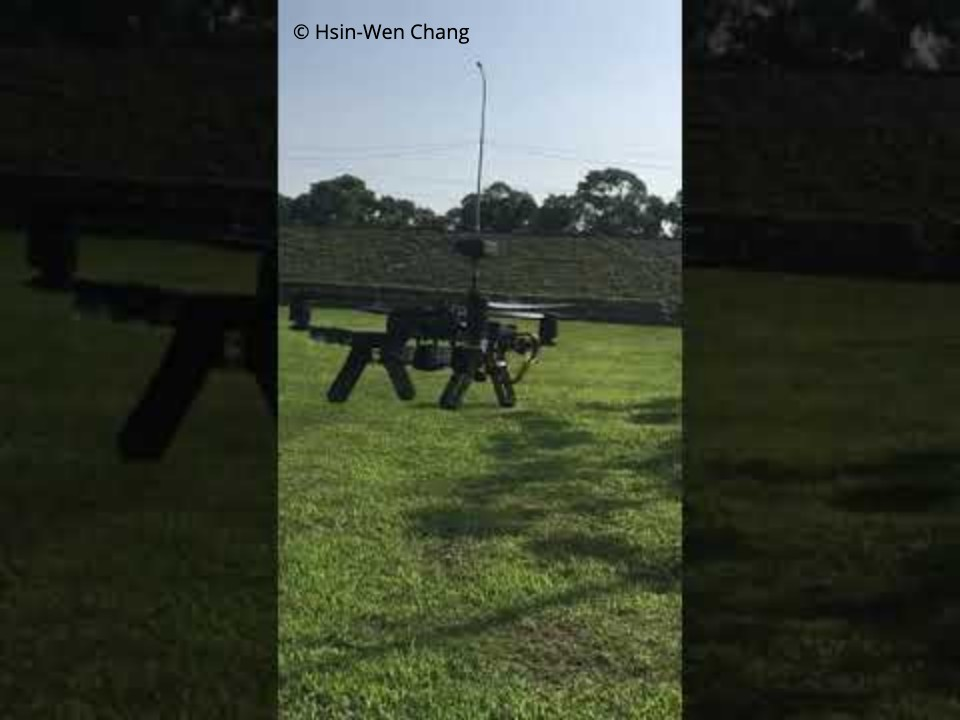
\includegraphics[width=\linewidth]{aero.jpeg}
      \caption{Intel aero Flying Car.}
      \label{fig:robot1}
\end{figure}
\begin{figure}[thpb]
      \centering
      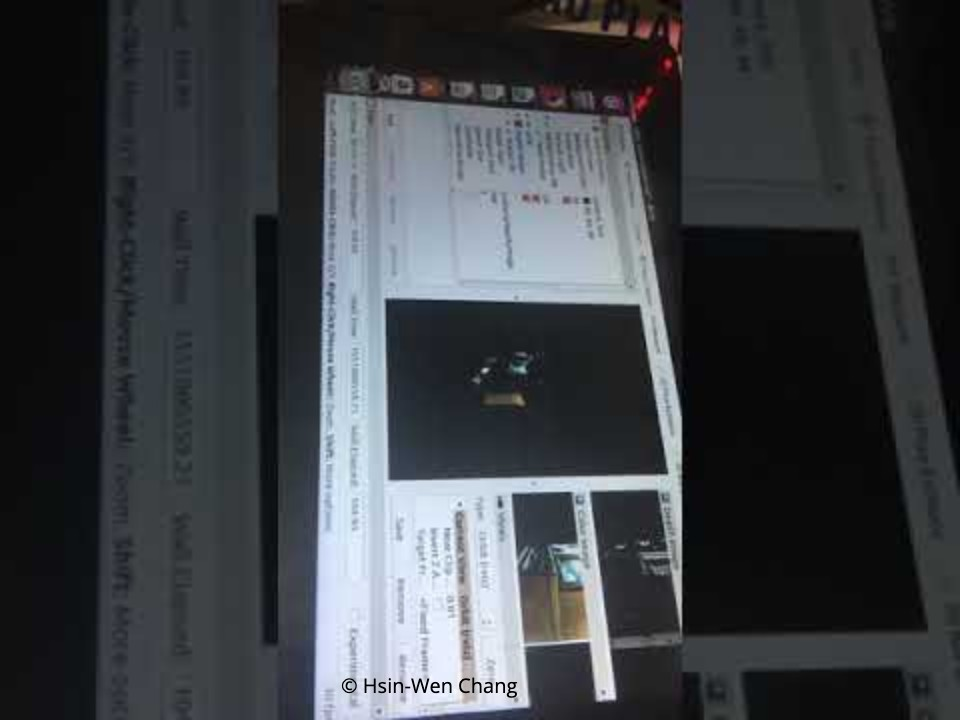
\includegraphics[width=\linewidth]{RTAB-Map.jpeg}
      \caption{Deploys RTAB-Map on the Intel aero Flying Car.}
      \label{fig:robot1}
\end{figure}

\bibliography{bib}
\bibliographystyle{ieeetr}

\end{document}
